\documentclass[]{beamer}
% https://github.com/tbagrel1/latex_resources
\usepackage{tbagrelbeamer}
\usepackage{beamerstylebluesky}
\usepackage{pgfplots}

\newcommand{\btf}{\tt{brain\_tumor\_factory}}
\newcommand{\btn}{\tt{brain\_tumor\_nn}}
\newcommand{\btnt}{\tt{brain\_tumor\_nn2}}
\newcommand{\ca}[1]{\tt{\alert{#1}}}
\newcommand{\icdc}[1]{\alert{$\pm{}[$}#1\alert{$]$}}
\usetikzlibrary{fadings}

\begin{document}

\title{Deep learning}
\subtitle{CNN and supervised learning}
\author{March 2019 @ TELECOM Nancy\\T. \sc{Bagrel}}
\date{}

\begin{frame}
  \titlepage{}
\end{frame}

% \begin{frame}
%   \frametitle{}
%   \framesubtitle{}
% \end{frame}

\begin{frame}
  \frametitle{Introduction}
  \framesubtitle{Interesting NN architectures (supervised)}
  \begin{block}{\bf{C}onvolutional \bf{N}eural \bf{N}etwork (CNN)}
    \begin{itemize}
      \item \alert{Supervised \tt{:(}}
      \item Most common architecture for image processing
      \item Position-invariant feature extraction (with shared weights)
      \item Very efficient
    \end{itemize}
  \end{block}
\end{frame}
\begin{frame}
  \frametitle{Introduction}
  \framesubtitle{Interesting NN architectures (unsupervised)}
  \begin{block}{\bf{R}estricted \bf{B}oltzmann \bf{M}achine (RBM)}
    \begin{itemize}
      \item \alert{Unsupervised!}
      \item General feature extraction
      \item Basic block of \bf{D}eep \bf{B}elief \bf{N}etworks
    \end{itemize}
  \end{block}
  \begin{block}{\bf{A}uto\bf{e}ncoders (AE)}
    \begin{itemize}
      \item \alert{Unsupervised!}
      \item Can be used for denoising
      \item Can be used for general feature extraction
    \end{itemize}
  \end{block}
\end{frame}

\begin{frame}
  \frametitle{Autoencoders}
  \framesubtitle{Structure and principle}
  \begin{block}{Principle}
    \begin{itemize}
      \item \alert{Simple} : reproduce the input at the output
      \item \alert{How} : pass the input (image) through the NN, compute error from $\text{diff}(I, O)$, adjust weights with GD
    \end{itemize}
  \end{block}
  \begin{exampleblock}{Feature extraction}
    \alert{Bottleneck} : ``center'' of the NN where there is the lowest number of neurons. Activation in the ``bottleneck'' for a given input (image) represents its compressed form.
  \end{exampleblock}
\end{frame}

\begin{frame}
  \frametitle{Autoencoders}
  \framesubtitle{Denoising}
  \begin{center}
    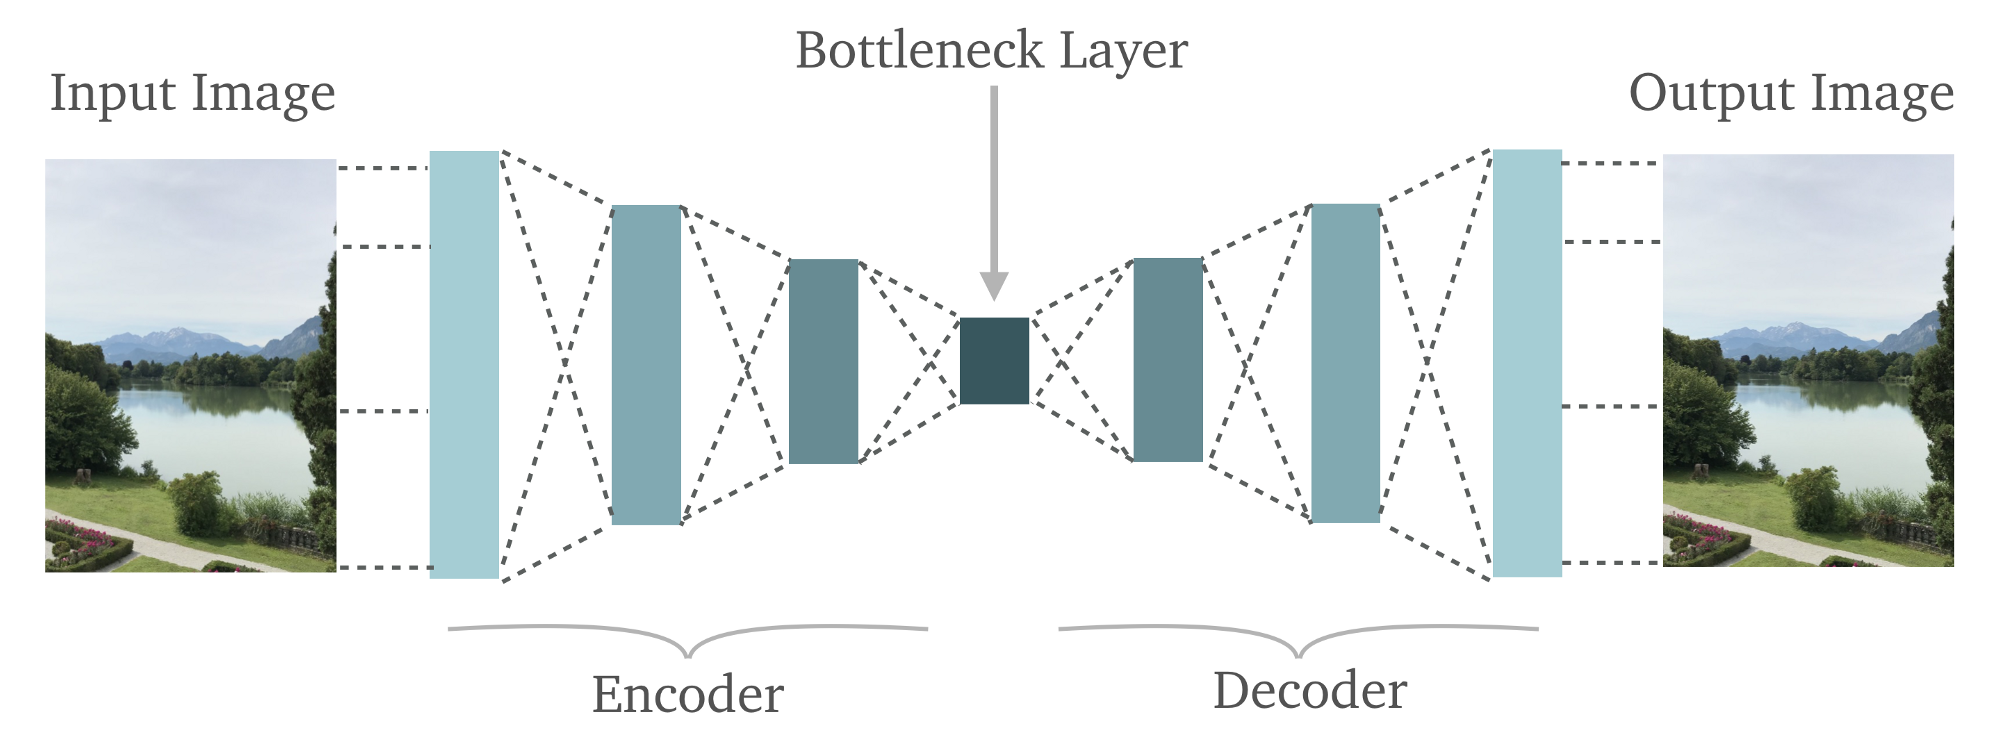
\includegraphics[width=\linewidth]{resources/autoencoder}
    \captionof{figure}{Autoencoder with feature extraction purpose}
  \end{center}

  \begin{exampleblock}{Denoising}
    Denoising can be achieved with roughly the same architecture
  \end{exampleblock}

\end{frame}

\begin{frame}
  \frametitle{CNN Components}
  \framesubtitle{Gradient Descent}
  \begin{center}
    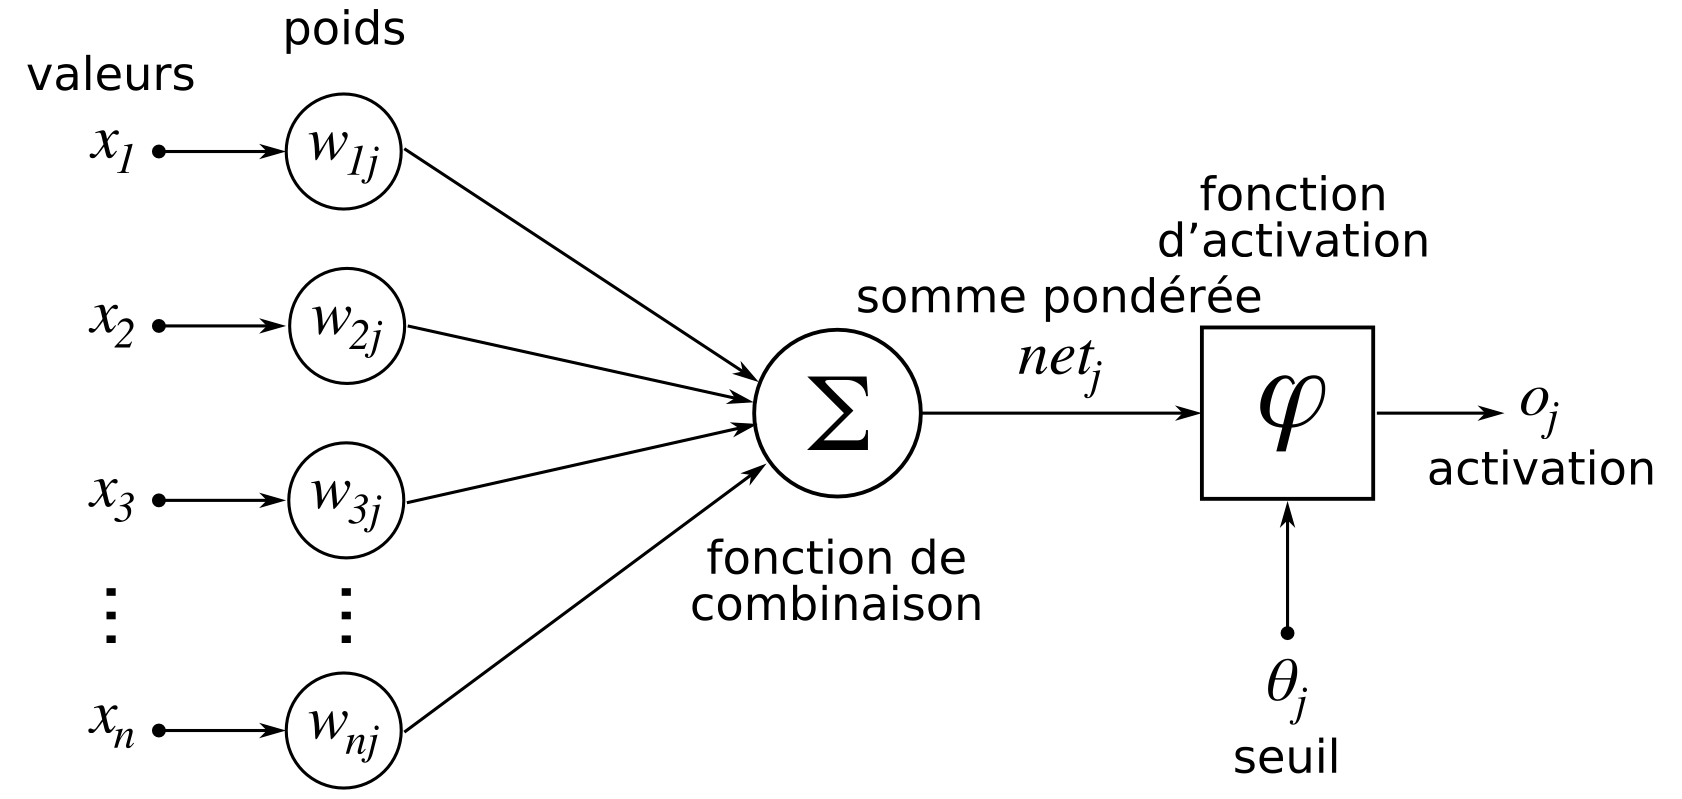
\includegraphics[width=\linewidth]{resources/perceptron}
    \captionof{figure}{Neuron (perceptron) schema}
  \end{center}
\end{frame}

\begin{frame}
  \frametitle{CNN Components}
  \framesubtitle{Gradient Descent}
  \begin{block}{Problem solved by GD}
    In which direction do we need to update our weights to minimize the error?
  \end{block}
  \begin{exampleblock}{Last layer neuron $n$ situation}
    $E$: error, $L$: loss function, $e$: expected value, $o$: obtained value, $\phi$: activation function, $x_{n, \cdot}$: inputs for the last layer neuron, $w_{n, \cdot}$: weights for the last layer neuron
    \begin{IEEEeqnarray}{rCl}
      E &=& L(e, o) \\
        &=& L\left(e,~~~\phi\left(\sum_k x_{n, k} w_{n, k}\right)\right)
    \end{IEEEeqnarray}
  \end{exampleblock}
\end{frame}

\begin{frame}
  \frametitle{CNN Components}
  \framesubtitle{Gradient Descent}
  \begin{exampleblock}{What we need to know}
    \begin{itemize}
      \item \alert{loss function} $L(e, o)$ and $\dfrac{\partial{}L}{\partial{o}}$
      \item \alert{activation function} $\phi(r)$ and $\dfrac{\mrm{d}\phi}{\mrm{d}r}$
    \end{itemize}
  \end{exampleblock}
  \begin{exampleblock}{What we can compute}
    With the \alert{chain rule}, we can compute $\dfrac{\partial{}E}{\partial{}w_{n, k}}(e, o) \quad (\forall k)$
  \end{exampleblock}
\end{frame}

\begin{frame}
  \frametitle{CNN Components}
  \framesubtitle{Gradient descent and adjustment made}
  \begin{block}{Weights adjustment ($\alpha$ : learning rate)}
    \[ w_{n, k} \longleftarrow w_{n, k} - \alpha \cdot \dfrac{\partial{}E}{\partial{}w_{n, k}}(e, o) \]
  \end{block}
  \begin{center}
    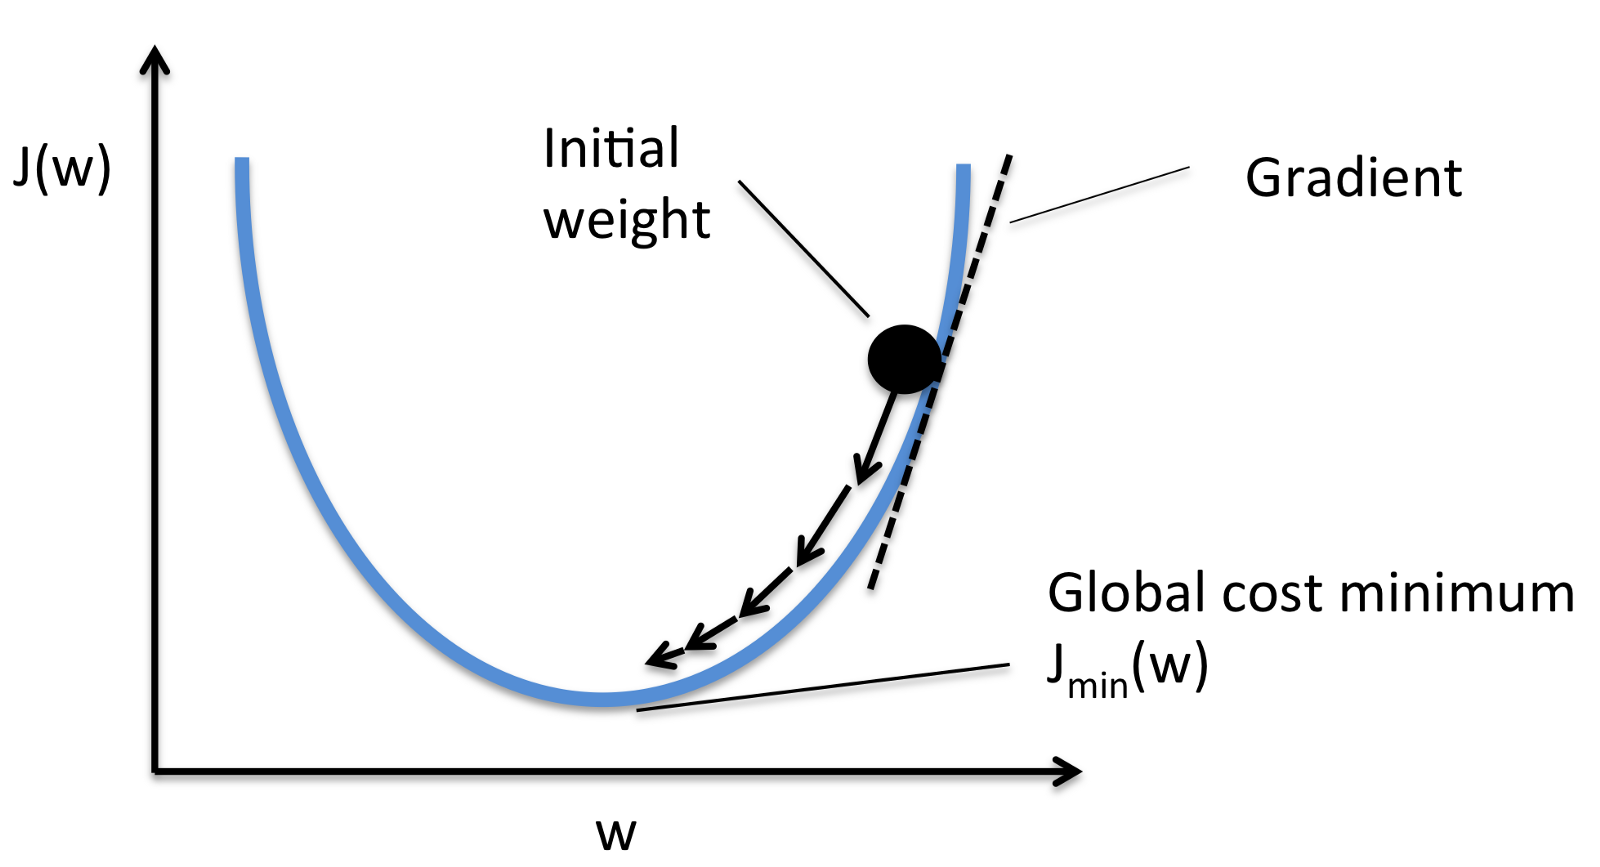
\includegraphics[width=0.8\linewidth]{resources/gd}
  \end{center}
\end{frame}

\begin{frame}
  \frametitle{CNN Components}
  \framesubtitle{Learning rate and advanced adjustment methods}
  \begin{center}
    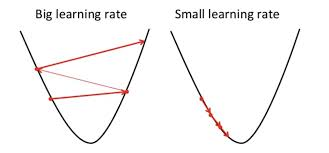
\includegraphics[width=\linewidth]{resources/big_vs_small_lr}
    \captionof{figure}{Importance of an appropriate learning rate}
  \end{center}
\end{frame}

\begin{frame}
  \frametitle{CNN Components}
  \framesubtitle{Advanced adjustment methods}
  Called optimizers in \alert{TensorFlow}
  \begin{block}{Roles}
    \begin{itemize}
      \item Try to prevent staying in a non-global local minima during learning
      \item \alert{Examples} : Nesterov Momentum, Adam\ldots{}
    \end{itemize}
  \end{block}

  \begin{exampleblock}{Used in my NNs}
    I use Nesterov's momentum: \tt{optimizers.SGD(nesterov=True, momentum=M)}\\ because it's recommended on most tutorials
  \end{exampleblock}
\end{frame}

\begin{frame}
  \frametitle{CNN Components}
  \framesubtitle{GD vs SGD vs BGD}
  Each one is a different manner to apply Gradient Descent
  \begin{block}{Differences}
    \begin{itemize}
      \item \alert{(basic) Gradient Descent} : weights are updated after every epoch (whole dataset pass) $\to$ \alert{very costly} but more stable than SGD!
      \item \alert{Stochastic Gradient Descent} : weights are updated after \alert{every} sample $\to$ \alert{very fast}!
      \item \alert{Batch Gradient Descent} : weights are updated after $N$ samples ($10 \le N \le 100$: batch size) $\to$ \alert{best of both worlds!}
    \end{itemize}
  \end{block}
\end{frame}

\begin{frame}
  \frametitle{CNN Components}
  \framesubtitle{Convolutional layer}
  The (3D) \alert{dot product} between the \alert{filter weights} and an \alert{input image zone} of the same size/shape gives an activation value. Doing this operation for all possible image zones (with \bf{overlap}) gives the \alert{activation map} for this filter.

  \it{It explains the position invariance of feature extraction for CNNs!}
  \begin{center}
    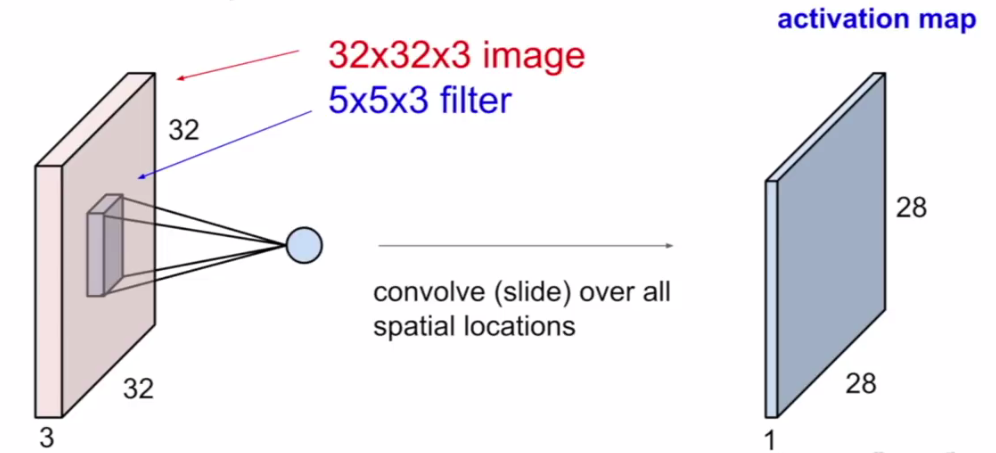
\includegraphics[width=0.8\linewidth]{resources/conv_1}
  \end{center}
\end{frame}

\begin{frame}
  \frametitle{CNN Components}
  \framesubtitle{Convolutional layer}
  A \alert{convolutional layer} is composed of several filters, each one with its \alert{own weights}. Hence, the output of the convolutional layer is a \alert{stack of activation maps} (one for each filter)
  \begin{center}
    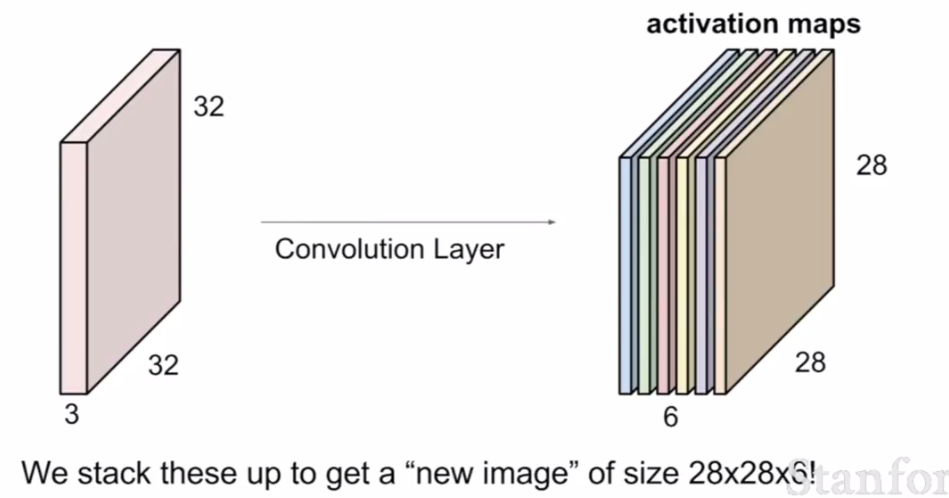
\includegraphics[width=0.8\linewidth]{resources/conv_2}
  \end{center}
\end{frame}

\begin{frame}
  \frametitle{CNN Components}
  \framesubtitle{Pooling layer}
  A \alert{pooling layer} is used to downsize/down-sample its input. \alert{All} the values in a zone of the input volume results in \alert{one} value in the output volume, by application of a simple function. Input zones \bf{must not overlap} here!

  A very common example is the \it{max pooling} 2 x 2:
  \begin{center}
    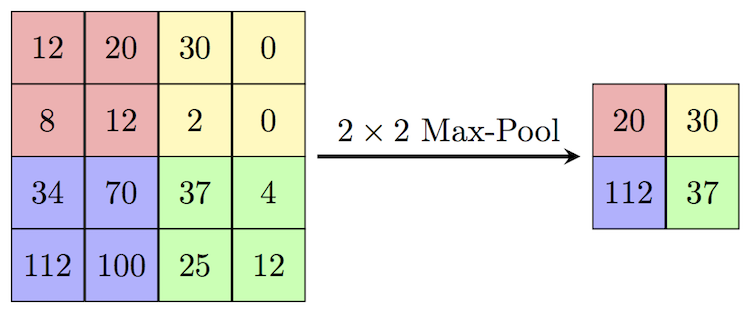
\includegraphics[width=\linewidth]{resources/pool}
  \end{center}
\end{frame}

\begin{frame}
  \frametitle{CNN Components}
  \framesubtitle{Output layer for classification}
  The output layer is used to extract classification information from a final dense/convolutional/pooling layer.
  \begin{block}{Types}
    \begin{itemize}
      \item For binary classification: Dense layer with \alert{sigmoid} activation function and \alert{1} neuron (1 output value)
      \item For multiclass classification : Dense layer with \alert{softmax} activation function and \alert{$\text{Nb}_{\text{classes}}$} neurons, followed by a $\text{arg\_max}(\cdot\cdot\cdot)$ function
    \end{itemize}
  \end{block}
\end{frame}

\begin{frame}
  \frametitle{CNN Components}
  \framesubtitle{Loss function for classification}
  \alert{Cross entropy} (aka. Negative Log Likelihood) is the loss function used in classification, which works well with the \alert{sigmoid} or \alert{softmax} activation functions (output layer)
  \begin{center}
    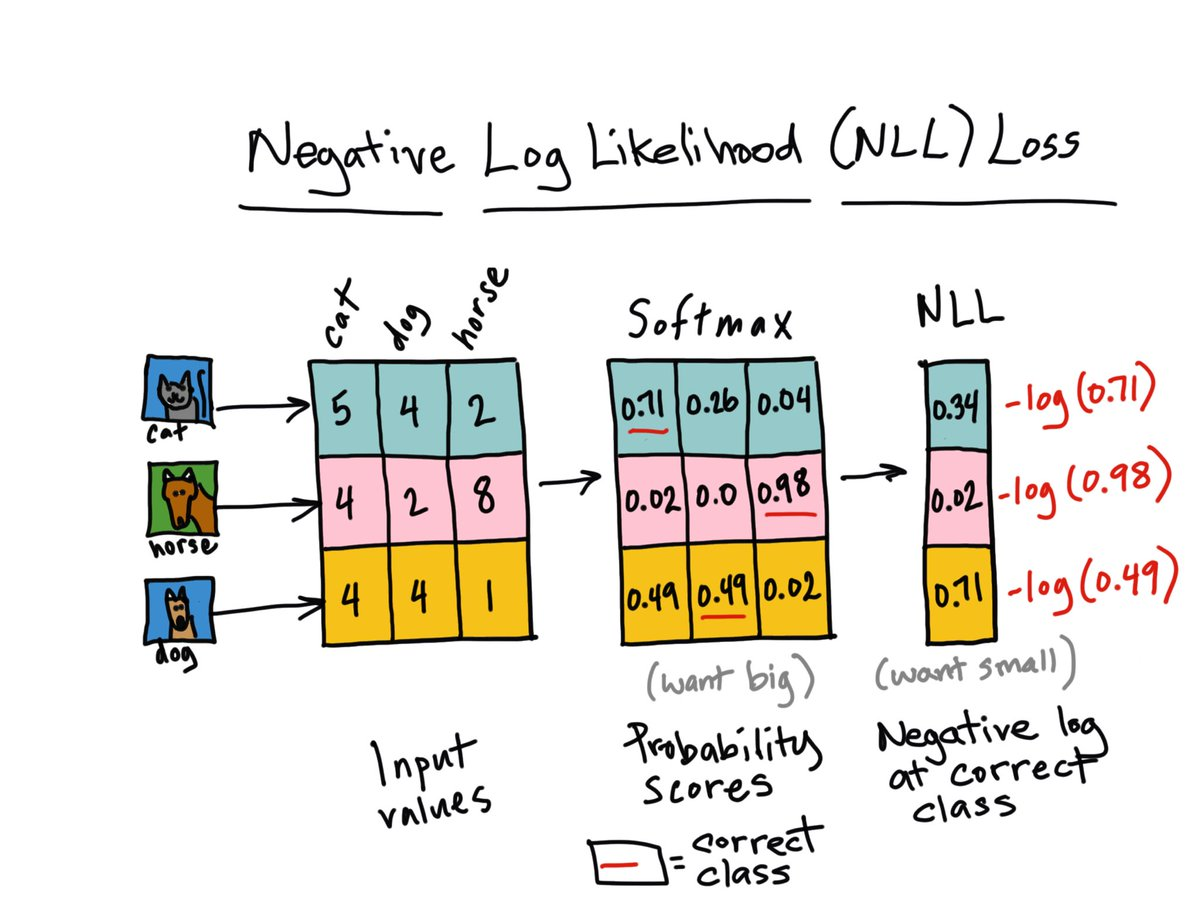
\includegraphics[width=0.7\linewidth]{resources/nll}
  \end{center}
\end{frame}

\begin{frame}
  \frametitle{CNN Components}
  \framesubtitle{CNN schema for multiclass}
  \begin{center}
    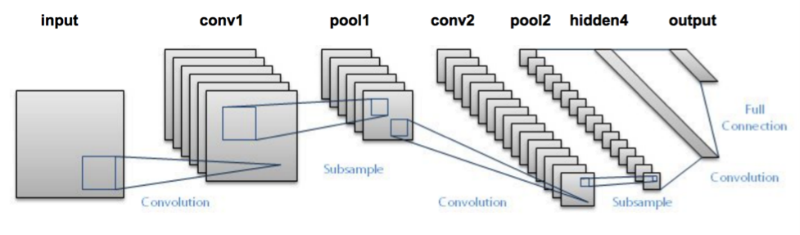
\includegraphics[width=\linewidth]{resources/cnn_schema}
    \captionof{figure}{CNN architecture}
  \end{center}
\end{frame}

\begin{frame}
  \frametitle{Medical imaging}
  \framesubtitle{Availability}
  \begin{block}{The issue}
    There are medical image datasets available online, but
    \begin{itemize}
      \item \alert{High resolution}
      \item Difficult to find the differencies or the good class for an \alert{untrained eye}
      \item File format and dataset organisation is not always \alert{normalized}
    \end{itemize}
  \end{block}
  \begin{exampleblock}{Examples}
    \begin{itemize}
      \item \alert{List of public datasets}: \url{bit.ly/2EOziVp}, \url{bit.ly/2u0Da0Q}
      \item \alert{Datasets}: \url{bit.ly/2F34jqb} (cancer cells), \url{bit.ly/2u99w9L} (neuroimaging), \url{bit.ly/2cGnNQL} (Alzheimer)\ldots{}
    \end{itemize}
  \end{exampleblock}
\end{frame}

\begin{frame}
  \frametitle{Medical imaging}
  \framesubtitle{What to do so?}
  \begin{block}{Requirements}
    \begin{itemize}
      \item Large dataset
      \item Low-res images (max. 256 x 256)
      \item Something which looks like medical images
    \end{itemize}
  \end{block}
  \begin{exampleblock}{Idea}
    Generate \alert{brain 2D images} and add random ``tumors'' on them
  \end{exampleblock}
  \begin{center}
    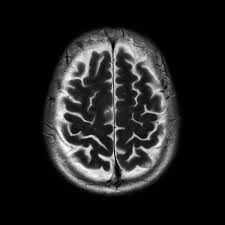
\includegraphics[width=1.8cm]{resources/brain_base}
  \end{center}
\end{frame}

\begin{frame}
  \frametitle{\btf}
  \framesubtitle{Let's get our hands dirty!}
  \begin{block}{How to generate?}
    Home-made C program: \alert{\btf}
    \begin{itemize}
      \item take a \alert{single} base image
      \item add tumor(s) randomly depending on the chosen scenario
      \item alter the resulting image, to ensure that each output image is a bit unique
    \end{itemize}
    Program size: $\simeq$ 500 LOC

    Output: $\simeq$ 1000 images/s

    Image size: \alert{96 x 128 x 1} (grayscale)
  \end{block}
\end{frame}

\tikzfading[name=fade out, inner color=transparent!0,
  outer color=transparent!100]

\begin{frame}[fragile]
  \frametitle{\btf}
  \framesubtitle{Creating tumors: \tt{tumor} function}
  \begin{block}{Instructions}
    Take a cirle of radius $R_{\text{area}}$, and put $n \in \itg{n_{\text{min}}, n_{\text{max}}}$ ``soft discs'' of radius $r_i \in [r_{\text{min}}, r_{\text{max}}]$ with their center placed randomly inside the chosen area
  \end{block}
  \begin{center}
    \begin{tikzpicture}[scale=0.5]
      \draw (0, 0) circle (4cm);
      \fill[path fading=fade out, color=alertTextColor] (0.3, 0.4) circle (3cm);
      \fill[path fading=fade out, color=alertTextColor] (2.3, -1.9) circle (1.75cm);
      \fill[path fading=fade out, color=alertTextColor] (-1.2, 2.54) circle (2.22cm);
      \fill[path fading=fade out, color=alertTextColor] (-0.98, -1.44) circle (1.48cm);
    \end{tikzpicture}
  \end{center}
\end{frame}

\begin{frame}
  \frametitle{\btf}
  \framesubtitle{Altering the resulting image: \tt{alter\_full} function}
  \begin{block}{Alterations}
    \begin{itemize}
      \item \ca{shrink}: shrink the image on x-axis and/or y-axis
      \item \ca{move}: shift the image on x-axis and/or y-axis
      \item (\ca{ghost\_blur~\tss{0.1\%}}): simulate motion blur on a shot
      \item \ca{alter\_contrast}: \icdc{brightness range}, with custom ``brightness center''
      \item \ca{alter\_shade}: global flat \icdc{brightness}
      \item \ca{alter\_rdc}: per-pixel flat random \icdc{brightness}
    \end{itemize}
  \end{block}

  For each image, alterations parameters are random numbers taken from a \alert{uniform} or \alert{normal} distribution
\end{frame}

\begin{frame}
  \frametitle{\btf}
  \framesubtitle{Base image}
  \begin{center}
    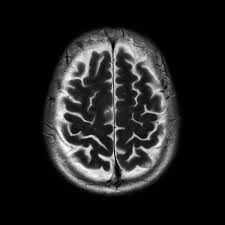
\includegraphics[width=5.5cm]{resources/brain_base}
  \end{center}
\end{frame}

\begin{frame}
  \frametitle{\btf}
  \framesubtitle{Altered images}
  \begin{minipage}{\linewidth}
    \begin{center}
      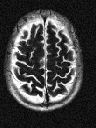
\includegraphics[width=2.55cm]{resources/z1}
      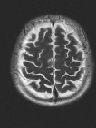
\includegraphics[width=2.55cm]{resources/z2}
      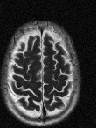
\includegraphics[width=2.55cm]{resources/z3}
      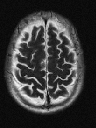
\includegraphics[width=2.55cm]{resources/z4}
    \end{center}
  \end{minipage}
  \begin{minipage}{\linewidth}
    \begin{center}
      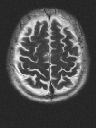
\includegraphics[width=2.55cm]{resources/z5}
      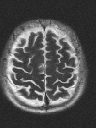
\includegraphics[width=2.55cm]{resources/z6}
      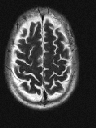
\includegraphics[width=2.55cm]{resources/z7}
      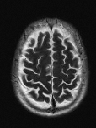
\includegraphics[width=2.55cm]{resources/z8}
    \end{center}
  \end{minipage}
\end{frame}

\begin{frame}
  \frametitle{\btf}
  \framesubtitle{Syndrome A}
  \begin{block}{Description}
    \begin{itemize}
      \item \alert{$\itg{1, 2}$} big tumor(s)
      \item \alert{$\itg{0, 2}$} medium tumor(s)
    \end{itemize}
  \end{block}
  \begin{center}
    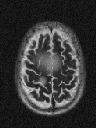
\includegraphics[width=3.2cm]{resources/a1e}
  \end{center}
\end{frame}

\begin{frame}
  \frametitle{\btf}
  \framesubtitle{Syndrome B}
  \begin{block}{Description}
    \begin{itemize}
      \item \alert{$\itg{4, 8}$} medium tumor(s)
      \item \alert{$\itg{0, 3}$} small/tiny tumor(s)
    \end{itemize}
  \end{block}
  \begin{center}
    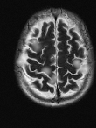
\includegraphics[width=3.2cm]{resources/b1e}
  \end{center}
\end{frame}

\begin{frame}
  \frametitle{\btf}
  \framesubtitle{Syndrome C}
  \begin{block}{Description}
    \begin{itemize}
      \item only \alert{$\itg{20, 48}$} small/tiny tumor(s)
    \end{itemize}
  \end{block}
  \begin{center}
    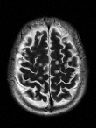
\includegraphics[width=3.2cm]{resources/c1e}
  \end{center}
\end{frame}

\begin{frame}
  \frametitle{\btf}
  \framesubtitle{Guess game: EASY mode}
  \begin{minipage}{\linewidth}
    \begin{center}
      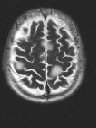
\includegraphics[width=2.55cm]{resources/b2e}
      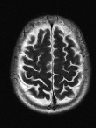
\includegraphics[width=2.55cm]{resources/z1e}
      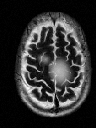
\includegraphics[width=2.55cm]{resources/a2e}
      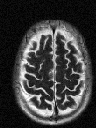
\includegraphics[width=2.55cm]{resources/z3e}
    \end{center}
  \end{minipage}
  \begin{minipage}{\linewidth}
    \begin{center}
      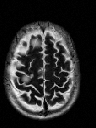
\includegraphics[width=2.55cm]{resources/b4e}
      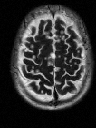
\includegraphics[width=2.55cm]{resources/c2e}
      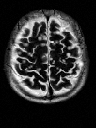
\includegraphics[width=2.55cm]{resources/c3e}
      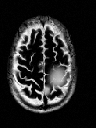
\includegraphics[width=2.55cm]{resources/a4e}
    \end{center}
  \end{minipage}
\end{frame}

\begin{frame}
  \frametitle{\btf}
  \framesubtitle{Guess game: HARD mode}
  \begin{block}{Observation}
    It turns out that it's kinda easy to find the correct syndrome type, isn't it?

    Let's try the \alert{HARD} mode then (more realistic) 
\includegraphics[height=12pt]{resources/devil}
  \end{block}

  \begin{exampleblock}{HARD mode specifications}
    \begin{itemize}
      \item Tumor opacity \alert{greatly} reduced
      \item Tumor size reduced a bit
    \end{itemize}
  \end{exampleblock}

  The \alert{base image} will always be placed on the \alert{LEFT} of the image whose type must be determined
\end{frame}

\begin{frame}
  \frametitle{\btf}
  \framesubtitle{Guess game: HARD mode}
  \begin{minipage}{\linewidth}
    \begin{center}
      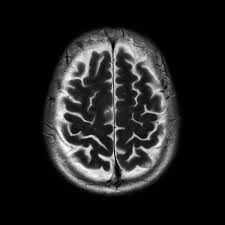
\includegraphics[width=4.2cm]{resources/brain_base}
      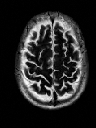
\includegraphics[width=4.2cm]{resources/c2}
    \end{center}
  \end{minipage}
  \pause
  \begin{block}{Answer}
    Syndrome C
  \end{block}
\end{frame}

\begin{frame}
  \frametitle{\btf}
  \framesubtitle{Guess game: HARD mode}
  \begin{minipage}{\linewidth}
    \begin{center}
      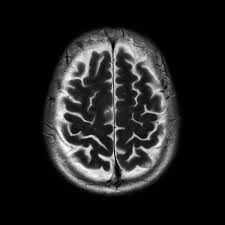
\includegraphics[width=4.2cm]{resources/brain_base}
      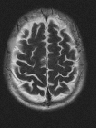
\includegraphics[width=4.2cm]{resources/a2}
    \end{center}
  \end{minipage}
  \pause
  \begin{block}{Answer}
    Syndrome A
  \end{block}
\end{frame}

\begin{frame}
  \frametitle{\btf}
  \framesubtitle{Guess game: HARD mode}
  \begin{minipage}{\linewidth}
    \begin{center}
      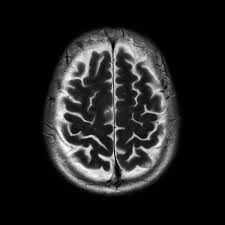
\includegraphics[width=4.2cm]{resources/brain_base}
      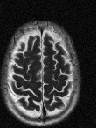
\includegraphics[width=4.2cm]{resources/z3}
    \end{center}
  \end{minipage}
  \pause
  \begin{block}{Answer}
    Z (healthy patient)
  \end{block}
\end{frame}

\begin{frame}
  \frametitle{\btf}
  \framesubtitle{Guess game: HARD mode}
  \begin{minipage}{\linewidth}
    \begin{center}
      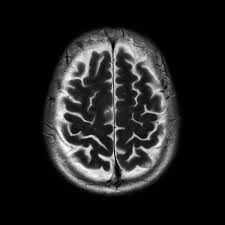
\includegraphics[width=4.2cm]{resources/brain_base}
      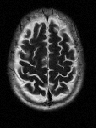
\includegraphics[width=4.2cm]{resources/b2}
    \end{center}
  \end{minipage}
  \pause
  \begin{block}{Answer}
    Syndrome B
  \end{block}
\end{frame}

\begin{frame}
  \frametitle{\btf}
  \framesubtitle{Guess game: HARD mode}
  \begin{minipage}{\linewidth}
    \begin{center}
      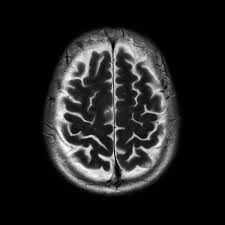
\includegraphics[width=4.2cm]{resources/brain_base}
      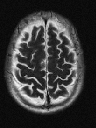
\includegraphics[width=4.2cm]{resources/z4}
    \end{center}
  \end{minipage}
  \pause
  \begin{block}{Answer}
    Z (healthy patient)
  \end{block}
\end{frame}

\begin{frame}
  \frametitle{\btf}
  \framesubtitle{Guess game: HARD mode}
  \begin{minipage}{\linewidth}
    \begin{center}
      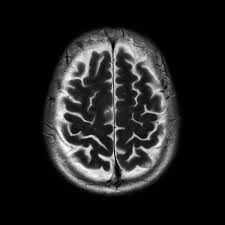
\includegraphics[width=4.2cm]{resources/brain_base}
      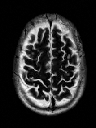
\includegraphics[width=4.2cm]{resources/c3}
    \end{center}
  \end{minipage}
  \pause
  \begin{block}{Answer}
    Syndrome C
  \end{block}
\end{frame}

\begin{frame}
  \frametitle{\btf}
  \framesubtitle{Guess game: HARD mode}
  \begin{block}{Observation}
    Not so easy this time? 
\includegraphics[height=12pt]{resources/devil}
  \end{block}

  \vfill

  \begin{center}
    \Large
    Let's see what \alert{deep learning} can do
  \end{center}

  \vfill
\end{frame}

\begin{frame}
  \frametitle{\btn}
  \framesubtitle{Description}
  \begin{block}{Framework}
    \begin{itemize}
      \item DL4j / ScalNet (Scala)
      \item not really fast (afterwards)
      \item Keras-like API
    \end{itemize}
  \end{block}
  \begin{exampleblock}{Architecture}
    \begin{itemize}
      \item 3 \tt{Conv2D} (\tt{MaxPooling2D} inbetween): 16 64 256
      \item \tt{Dense} 1024
      \item GD (BGD) with Nesterov Momentum
      \item (adapted from MNIST NN examples)
    \end{itemize}
  \end{exampleblock}
\end{frame}

\begin{frame}
  \frametitle{\btn}
  \framesubtitle{Description}
  \begin{block}{Issue (after 2 hours learning)}
    \begin{itemize}
      \item Accuracy blocked at 0.25
      \item loss wasn't decreasing
      \item a \alert{single type} predicted everytime
    \end{itemize}
  \end{block}
  \begin{exampleblock}{Why (afterwards)}
    \begin{itemize}
      \item I didn't wait long enough
      \item 3 Conv layer NN + slow framework didn't help much neither
      \item in addition, learning on mobile CPU (i7) is still slow
      \item (but afterwards) architecture wasn't really the issue
    \end{itemize}
  \end{exampleblock}
\end{frame}

% brain_tumor_nn2
% what can be achieved
% overfitting
% regularization
% underfitting
% easy then hard, why it seemed to be not working at the beginning
% evolutions of the nn

% image virtual augmentation not used here

% hardware & software
% dl4j
% cpu vs gpu
% tensorflow
% futur equipment ?

% credits

\begin{frame}
  \frametitle{}
  \framesubtitle{}
\end{frame}

\end{document}
